\documentclass[unicode,11pt,a4paper,oneside,numbers=endperiod,openany]{scrartcl}

\input{assignment.sty}
\begin{document}


\setassignment
\setduedate{27.11.2020 23:59 (midnight)}

\serieheader{High-Performance Computing Lab}{Fall 2020}{Student: Gabriele Berra}{Discussed with: -}{Solution for Project 6}{}
\newline

\assignmentpolicy

\section{Ring maximum using MPI [10 Points]}
In this first exercise, I implemented the function \textit{max\_ring.c}, parallelized with MPI. Similarly to what we did in class, I firstly defined the left and right neighbour and the value of the function  
\begin{equation}\label{eq:maxEx1}
	\text{max} = 3 * \text{process\_rank}_i \mod(2 * \text{communicator\_size}) 
\end{equation}
for each processor. Since we have to run the function with 4 processors, we know that the global maximum of Eq. \ref{eq:maxEx1} is reached in the processor 2 with $\max = 6$. In the main body of the function, on one hand, each processor, with the MPI routine \texttt{MPI\_Send}, exchanges its own maximum with the next processor. On the other hand, with the MPI routine \texttt{MPI\_Recv}, the processor that receives the data checks if its own maximum is bigger or lower than the maximum that it has received and keeps the bigger one. Repeating this routine in a circular manner as many times as the number of processors (i.e., 4 times in this example) gives the following results:

\begin{lstlisting}[language = bash, backgroundcolor=\color{gray!20}]
Process 0:		Max = 6
Process 2:		Max = 6
Process 3:		Max = 6
Process 1:		Max = 6
\end{lstlisting}
 Of course, every time we run the script the order of the processes will change. In what follows I reported the main body of the function \textit{max\_ring.c}.

\lstinputlisting[frame=single, breaklines=true, tabsize=3, showstringspaces=false, firstline=53 ,lastline=71, language=C]{code/max_ring.c}


\section{Ghost cells exchange between neighboring processes [20 Points]}
For this second exercise we have to parallelize with MPI the exchange of ``ghost cells" between adjacent processors in a defined grid. The input data on which we have to work is a $(6+2)\times(6+2)$ matrix associated with each processors, in which each entry has value equal to the rank of the processor. 
The first step is to create a Cartesian communicator of dimension $4\times 4$ (which is a sort of matrix for the processors) with periodic boundaries: this means that the processor 0 - which is in position $(0,0)$ - can communicate with processor 3 and processor 12 on the left and top respectively. In order to find - for each processor - the top, bottom, left and right neighbours, we have to use the MPI routine \texttt{MPI\_Cart\_shift} which, given a shift direction and the amount of ``cells" to be shifted, returns the source and destination rank. In our case, to find the left and right neighbour we call the function as follows:

\lstinputlisting[frame=single, breaklines=true, tabsize=3, showstringspaces=false, firstline=92 ,lastline=92, language=C]{code/ghost.c}
which shifts on the $x$ axis (second input) of 1 cell (third input). Similarly, to find the top and bottom neighbour we use:
\lstinputlisting[frame=single, breaklines=true, tabsize=3, showstringspaces=false, firstline=93 ,lastline=93, language=C]{code/ghost.c}
which, in this case, shifts on the $y$ axis - i.e., vertically - of 1 cell.\\ Now that we know the neighbours of each processor, we have to exchange the correct data between them. We know that, since C stores data in row-major order, we have no problem in exchanging rows of a matrix because the data are contiguous in memory. The problem occurs when we want to exchange data that are not contiguous in memory. Fortunately, MPI gives us the routine \texttt{MPI\_Type\_vector} which creates a vector-type object. In order to use it in the correct manner, we first have to understand how it works. As input it accepts:

\begin{itemize}
	\item \textit{count}: number of blocks that we want to send;
	\item \textit{blocksize}: dimension of the block (in our case, since we want to send only one column of doubles, it is equal to 1);
	\item \textit{stride}: distance in memory between elements that we want to send;
	\item \textit{type}: type of the item that we want to send.
\end{itemize}

The last element in \texttt{MPI\_Type\_vector} is the output. Now we have created only a structure without any data inside it. When we use it in \texttt{MPI\_Send}, what it does is to take \textit{count} elements with distance from each other equal to \textit{stride}.\\ The last step is the exchange of the correct data between neighbours. In order to do so, I used the MPI routine \texttt{MPI\_Send} and \texttt{MPI\_Recv} in which, for each processor, I specify the correct position of the data that has to be sent and the position in which the receiver has to put the data received. As explained before, I used the vector-type object only to exchange data between left and right neighbours. The code I implemented is the following:\\
\lstinputlisting[frame=single, breaklines=true, tabsize=3, showstringspaces=false, firstline=101 ,lastline=121, language=C]{code/ghost.c}


\section{Parallelizing the Mandelbrot set using MPI [20 Points]}
With the aim of creating the Mandelbrot set using MPI, I firstly implemented the functions \textit{createPartition()}, \textit{updatePartition()} and \textit{createDomain()} in the file \textit{consts.h} as follows:
\lstinputlisting[frame=single, breaklines=true, tabsize=3, showstringspaces=false, firstline=43 ,lastline=135, language=C]{code/consts_mandel.h}

\begin{figure}[h!]
	\hspace{-1.5cm}\includegraphics[width=0.7\textwidth, angle=-90]{images/perf.ps}
	\vspace{1cm}
	\caption{Performance with different amount of processors}
	\label{fig:mandelPerf}
\end{figure}

As we can see in Fig. \ref{fig:mandelPerf}, the time for the computation of the Mandelbrot set using two processors is halved compared to the time using only one processor. In contrast, the difference between the time using 4 processors and the time using 8 processors is almost the same. We can notice that the computation time of, as example, processor 5, in the run using 16 processes, is exactly equal to the computation time of processor 9. This comparison can be extended to all the processes. The reason for this behaviour lies in the symmetry, with respect to the $x$ axis, of the Mandlebrot set. Thus, in the $4 \times 4$ grid reported in the left side of Fig.\ref{fig:procMatrix}, the pairs of processors with the same computation time are: (0 - 12), (1 - 13), (2 - 14), (3 - 15), (4 - 8),(5 - 9),(6 - 10) and, (7 - 11). We know that different areas of the Mandelbrot set require a different amount of time to be computed. In my opinion, the most interesting aspect - which is also the explanation of why this method of partitioning is not the most efficient - is the difference in terms of computation time between different processes. One of the most efficient ways to parallelize the Mandelbrot set consists in distributing the work among the processes in an equal way in terms of computation time.
\begin{figure}[h!]
	\centering
	\begin{subfigure}[b]{0.48\textwidth}
		\hspace{3cm}\begin{tikzpicture}
		\matrix[matrix of nodes,nodes={draw=gray, anchor=center, minimum size=1cm}, column sep=-\pgflinewidth, row sep=-\pgflinewidth] (A) {
		\Large{0} & \Large{1} & \Large{2} & \Large{3} \\
		\Large{4} & \Large{5} & \Large{6} & \Large{7} \\
		\Large{8} & \Large{9} & \Large{10} & \Large{11} \\
		\Large{12} & \Large{13} & \Large{14} & \Large{15}\\};
		\end{tikzpicture}
	\end{subfigure}
	\hfill
	\begin{subfigure}[b]{0.48\textwidth}
		\includegraphics[width=0.53\textwidth]{images/mandel.png}
	\end{subfigure}
	\caption{Left: grid of 16 processors. Right: Mandelbrot set}
	\label{fig:procMatrix}
\end{figure}


\section{Option A: Parallel matrix-vector multiplication and the power method [50 Points]}
With the aim of parallelizing the power method using MPI, I principally wrote two files. The first one, called \textit{consts.h}, contains the functions that we need in order to do the computations - e.g. matrix-vector multiplication or the norm of the vector - and the second one is the \textit{main.c} file, which uses the function in \textit{consts.h} and gives the timing for the computation of the power method. I decided to divide the work in the following way:
\begin{enumerate}
	\item Create a function called \textit{generateMatrix} which generates - initially - a test matrix with fixed entries for debugging purposes and then a matrix with random numbers;
	\item Create a function called \textit{generateVector} which generates - initially - a test vector with fixed entries for debugging purposes and then a vector with random numbers;
	\item Create a function called \textit{norm} which divides each entry of a given vector for its norm;
\end{enumerate}
After the creation of the above functions, I focused my effort on the parallelization of them using MPI. 
My first issue was the distribution of the rows of the matrix between the processors. In order to do so, instead of generating a complete matrix, I generated only the part of the matrix associated with each processor: thus, e.g., with a $8 \times 8$ matrix with $p = 2$, the processor 0 uses the function \textit{generateMatrix} to generate its own 16 entries (and the same happens for the second processor). The function is the following:
\lstinputlisting[frame=single, breaklines=true, tabsize=3, showstringspaces=false, firstline=66 ,lastline=81, language=C]{code/matVecMult/consts.h}

The second function that I implemented is \textit{generateVector} which, as the name suggests, generates a vector of length equal to the number of rows/colmuns of the matrix.
\lstinputlisting[frame=single, breaklines=true, tabsize=3, showstringspaces=false, firstline=168 ,lastline=182, language=C]{code/matVecMult/consts.h}

The most important function is the one that performs the matrix-vector multiplication using the MPI routines \texttt{MPI\_Bcast} and \texttt{MPI\_Gather} to exchange information between the processors. I implemented it in the following way:
\lstinputlisting[frame=single, breaklines=true, tabsize=3, showstringspaces=false, firstline=116 ,lastline=148, language=C]{code/matVecMult/consts.h}
The main function that puts all the pieces together is the following: 
\lstinputlisting[frame=single, breaklines=true, tabsize=3, showstringspaces=false, language=C]{code/matVecMult/main.c}

\subsection{Results}
In this section I will present the result of the parallel matrix-vector multiplication and of the power method, focusing my attention on both a strong and weak scaling analysis.
\begin{itemize}
	\item \textbf{Strong scaling analysis}: As we can see in the left part of Fig.\ref{fig:strongScal}, an increase in the number of processors used - initially - is extremely beneficial but, due to the increasing number of communication, the efficiency of using more processors decreases drastically from 16 to 32 processes and is more than halved from 32 to 64 (left part of Fig.\ref{fig:strongScal}). 
	\begin{figure}[h!]
		\centering 
		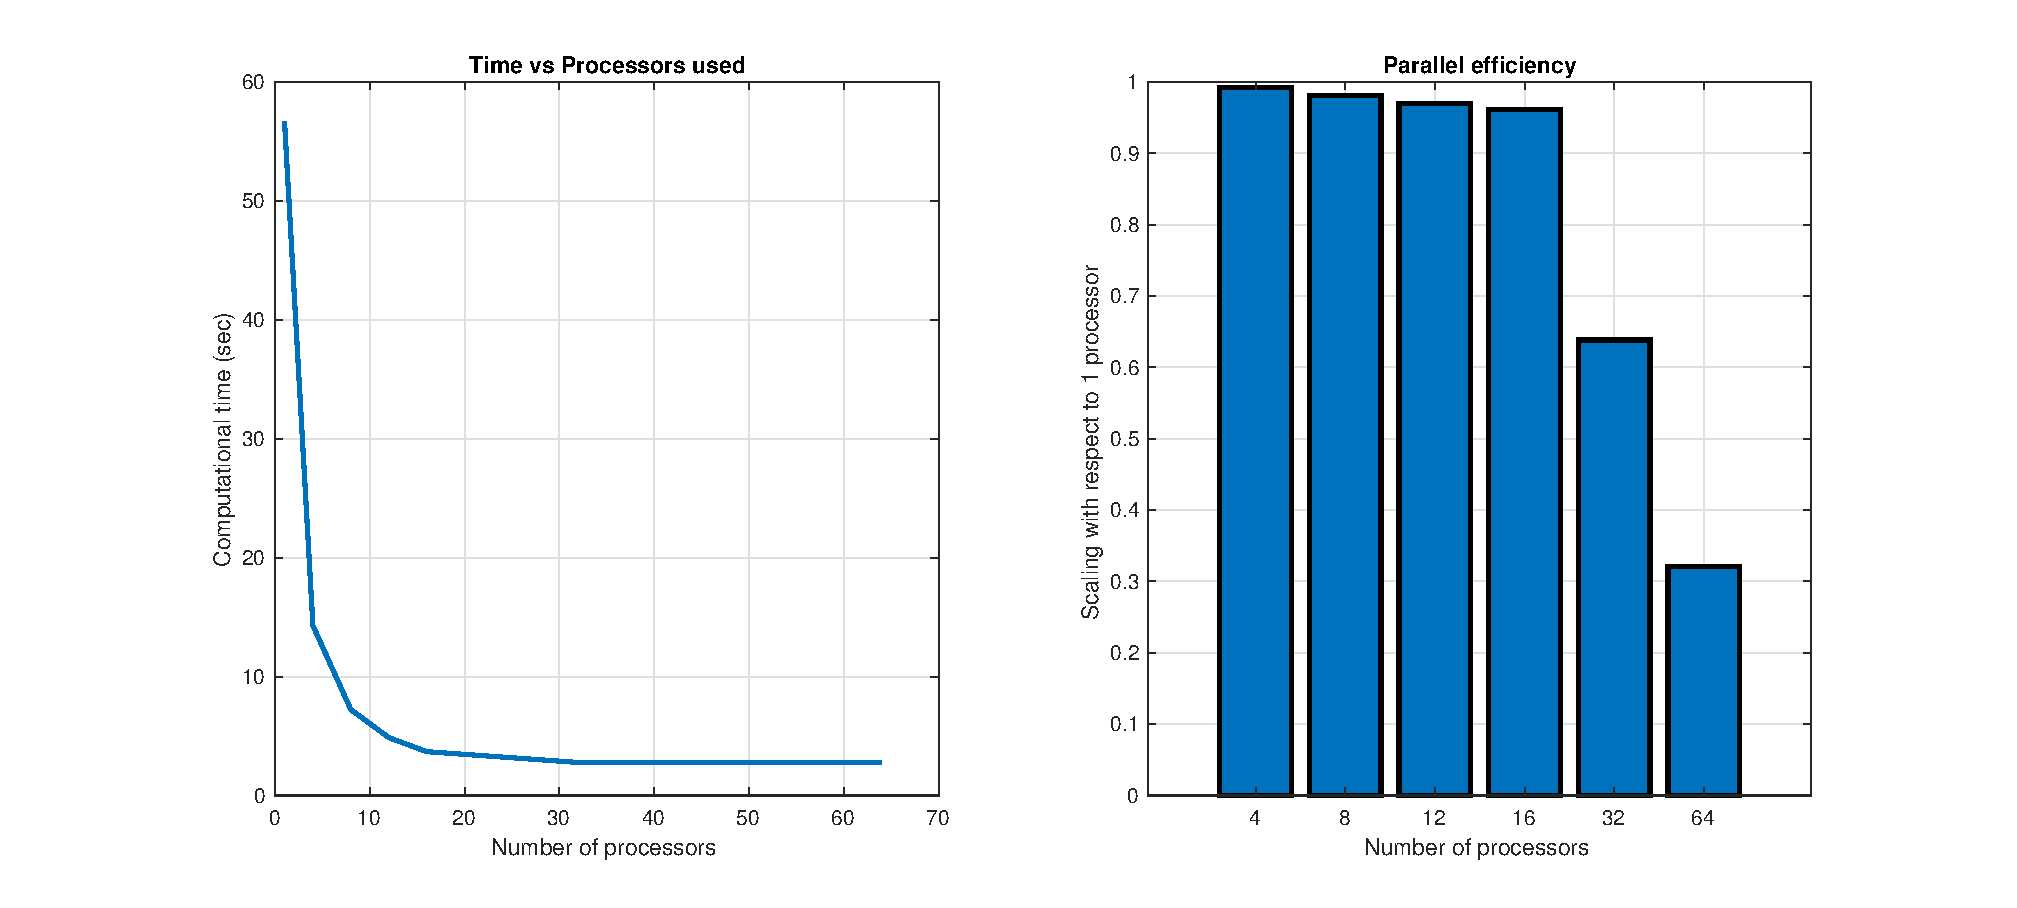
\includegraphics[width=\textwidth]{images/strong_scal.eps}
		\caption{Left: comparison between computation time and number of processors used. Right: parallel efficiency.}
		\label{fig:strongScal}
	\end{figure}
	\item \textbf{Weak scaling analysis}: In order to perform a weak scaling analysis, I run my code using different number of processors and matrix sizes which are proportional to $\sqrt{p}$. In Table \ref{tab:weakScal} I reported, for each number of processors used, the matrix size. I fixed the number of iterations of the power method to 100. In order to find the correct matrix size, I used the formula:
	 \begin{equation*}
	 	n=4000\sqrt{p}-\text{mod}(4000\sqrt{p}, p).
	 \end{equation*}
	\begin{table}[h!]
		\centering
		\begin{tabular}{|c|c|}
			\hline
			\# of proccessors & \# of rows/columns \\
			\hline
			1 & 4000\\
			\hline
			4 & 8000\\
			\hline
			8 & 11312\\
			\hline
			12 & 13848\\
			\hline
			16 & 16000\\
			\hline
			32 & 22624\\
			\hline
			64 & 32000\\
			\hline
		\end{tabular}
		\caption{Number of processor use associated with the correct matrix size.}
		\label{tab:weakScal}
	\end{table}
	In Fig.\ref{fig:weakScal}, I reported the results of the weak scaling analysis. As we can clearly see, when we increase the number of processors used from 32 to 64, the computational time is rocketing, due to the time needed for the communication between processors. In order to achieve the maximum of the performance, we have to take into consideration also the communication time which - for large matrices - has an enormous impact on the computation time.
	\begin{figure}[h!]
		\centering
		\includegraphics[width=\textwidth]{images/weak_scal}
	\caption{Weak scaling of matrix vector multiplication and power method}
	\label{fig:weakScal}
	\end{figure}
\end{itemize}

\subsection{How to run the main file}
In order to run the program on your laptop with, e.g., 4 processors, n = 4000, and k = 100, you have to follow the instructions reported below:
\begin{lstlisting}[language = bash, backgroundcolor=\color{gray!20}]
make
mpirun -np 4 ./main 4000 100
\end{lstlisting}

\end{document}
